\section{Supplementary Evidence and Protocol Details}

\subsection{Intervention-audit summary}
\begin{table*}[t]
\centering
\small
\begin{tabular}{p{0.19\textwidth}p{0.16\textwidth}p{0.19\textwidth}p{0.34\textwidth}}
\toprule
Analysis & Status & Paper use & Reason \\
\midrule
Aya layer-20 steering & Verified null control & Report as control & Development selected strength 0.0; 553 aligned baseline and nominally steered test predictions are byte-identical. \\
Aya layer-24 sweep & Unsupported & Exclude from confirmatory claims & Aggregate summary exists, but complete development record and paired selected-condition test predictions are unavailable. \\
Qwen layer-20 steering & Unusable for effect claims & Exclude & Direction is constructed from test examples; no matched test baseline; stored delta mixes development and test summaries. \\
mT5 Amharic sweep & Exploratory & Appendix & Raw generations show strength-dependent behavior, but direction/sweep are test-derived and omit a zero-strength baseline. \\
MT5/MT0 head ablations & Exploratory & Appendix & Head ordering is random rather than mechanistically targeted. \\
Llama steering & Unusable & Exclude & Stored values are estimated ablation proxies rather than generated outputs. \\
\bottomrule
\end{tabular}
\caption{Evidence status for recovered intervention artifacts.}
\label{tab:intervention-audit}
\end{table*}


\subsection{Exploratory Amharic steering sweep}

\begin{figure*}[t]
\centering
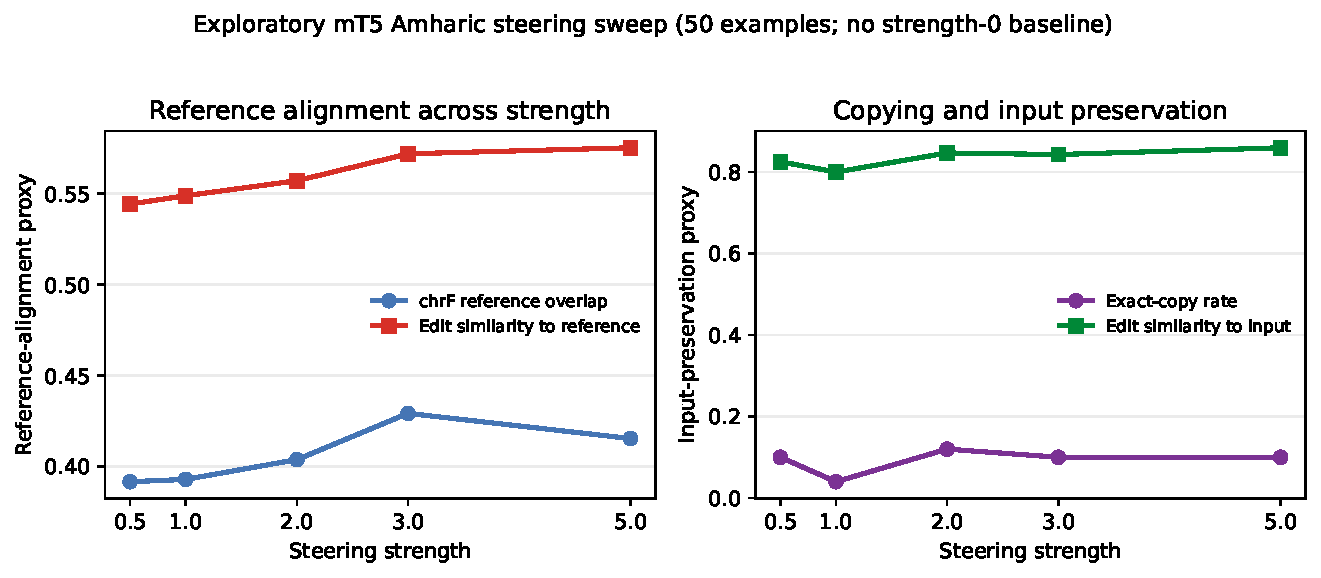
\includegraphics[width=0.9\textwidth]{figures/fig_mt5_amharic_exploratory_steering.pdf}
\caption{Exploratory mT5 Amharic steering sweep. Across 50 examples, five nonzero
intervention strengths produce distinct, non-empty, and unique outputs. The sweep is
exploratory because the archived direction and sweep use test-derived data, omit a
strength-zero baseline, lack independent non-toxicity measurement, and have no
confidence intervals or seed replication.}
\label{fig:amharic-sweep}
\end{figure*}

\subsection{Human-evaluation protocol}

The final supplementary package will include the annotation form, instructions,
sampling procedure, anonymized completed labels, agreement calculations, and
per-language counts after annotation is complete.

\subsection{SAE inventories}

The final supplementary package will include seed-specific SAE configuration details,
candidate feature inventories, and feature-interpretation examples. These materials
will be described as candidate analyses unless validated by aligned dictionaries and
causal interventions.
